%\chapter{Introdução}

\chapter{Introdução}

Este Trabalho de Conclusão de Curso (TCC) aborda o desenvolvimento de uma extensão Flutter que visa auxiliar os desenvolvedores no processo de criação de aplicações móveis acessíveis em Flutter. A motivação para este trabalho surge da crescente importância da inclusão e da acessibilidade no desenvolvimento de aplicações móveis, bem como da necessidade de simplificar e melhorar o processo de desenvolvimento de soluções acessíveis utilizando tecnologias modernas, como o Flutter.

O TCC foi desenvolvido seguindo uma metodologia baseada nas fases fundamentais da Engenharia de Software, incluindo análise (Engenharia de Requisitos), projeto, programação, testes e validação. Além disso, a execução do trabalho foi gerenciada utilizando a metodologia ágil, garantindo um desenvolvimento iterativo e incremental do projeto.

A introdução detalha o contexto, a problemática, os objetivos geral e específicos, a justificativa e a metodologia adotada no desenvolvimento do trabalho. Em seguida, o TCC é organizado em capítulos que abordam a revisão da literatura, o projeto e a implementação da extensão, os testes e a validação realizados com desenvolvedores e PCDs, e o gerenciamento do projeto. Por fim, as conclusões discutem os principais resultados, limitações e possíveis trabalhos futuros relacionados ao tema da acessibilidade em aplicações móveis.

\section{Problema}

A acessibilidade tem se tornado cada vez mais relevante no contexto do desenvolvimento de aplicações móveis, uma vez que possibilita a inclusão e a igualdade de oportunidades para pessoas com deficiência (PCDs). As aplicações móveis têm desempenhado um papel essencial no cotidiano das pessoas, e é imprescindível que elas sejam projetadas de forma inclusiva, garantindo uma experiência eficiente e satisfatória para todos os usuários. Neste cenário, o presente TCC se aplica ao desenvolvimento de aplicações móveis acessíveis utilizando o framework Flutter, que tem sido amplamente adotado devido à sua capacidade de criar aplicativos de alta qualidade e com desempenho otimizado para múltiplas plataforma. Contudo, o desenvolvimento de aplicações móveis acessíveis em Flutter ainda enfrenta desafios relacionados à complexidade e à necessidade de conhecimento especializado.

O problema abordado neste TCC é a dificuldade enfrentada pelos desenvolvedores ao implementar recursos de acessibilidade em aplicações móveis criadas com Flutter, em razão das lacunas de conhecimento e da complexidade inerente a essa tarefa. A solução proposta visa simplificar e tornar mais prática a criação de aplicações móveis acessíveis, contribuindo para a melhoria da experiência dos PCDs ao utilizar essas aplicações.

Para abordar este problema, serão investigadas as melhores práticas e técnicas disponíveis na literatura relacionadas à acessibilidade em aplicações móveis. Além disso, será desenvolvida uma aplicação de exemplo que demonstre a aplicabilidade das soluções propostas, servindo como referência para os desenvolvedores Flutter.

\subsection{Objetivo Geral}

O objetivo geral deste trabalho é apoiar o desenvolvimento de aplicativos móveis mais acessíveis. Para isso, visa-se criar uma extensão Flutter que facilite o processo de desenvolvimento de aplicações móveis acessíveis em Flutter para os desenvolvedores através da análise estática de código. A extensão fornecerá orientações e recomendações sobre a utilização de componentes e a aplicação de regras necessárias para cumprir com os requisitos de acessibilidade não funcionais. Através dessa abordagem, a extensão auxiliará os desenvolvedores a criar aplicativos mais inclusivos, melhorando a experiência dos PCDs ao utilizar essas aplicações.

Além disso, este trabalho visa aumentar a conscientização sobre a importância da acessibilidade no desenvolvimento de aplicações móveis. Para isso, serão publicados os requisitos de acessibilidade utilizados durante o desenvolvimento da extensão, a fim de promover uma compreensão mais ampla das melhores práticas e normas aplicáveis a essa área.

Dessa forma, a solução proposta contribui para resolver o problema apresentado ao facilitar a criação de aplicações móveis acessíveis em Flutter, fornecendo aos desenvolvedores as ferramentas e informações necessárias para atender aos requisitos de acessibilidade e, ao mesmo tempo, promovendo uma maior conscientização sobre a importância desse tema no contexto atual.

\subsection{Objetivos Específicos}

\subsubsection{Revisão da Literatura}

Realizar um mapeamentosistemático da literatura para identificar os requisitos não funcionais de acessibilidade necessários para aplicações móveis, permitindo estabelecer uma base sólida para o desenvolvimento da extensão proposta e garantir a aderência às melhores práticas e normas do campo.

\subsubsection{Projeto e Implementação da Extensão}

Desenvolver uma extensão Flutter que analise o código-fonte de aplicações móveis e forneça orientações e recomendações sobre a utilização de componentes e a aplicação de regras de acessibilidade. A extensão deverá ser integrada ao ambiente de desenvolvimento e ser capaz de identificar possíveis problemas de acessibilidade no código, sugerindo soluções e boas práticas para corrigi-los.

\subsubsection{Testes e Validação}

Realizar testes e validações da extensão com desenvolvedores e PCDs para avaliar a eficácia e a usabilidade da ferramenta. Os testes serão conduzidos em um ambiente controlado, permitindo identificar possíveis falhas e melhorias na extensão, bem como coletar feedbacks e sugestões para aprimorar a solução proposta.

\subsubsection{Documentar e Disseminar}

Documentar o processo de desenvolvimento da extensão, incluindo os requisitos de acessibilidade utilizados, as técnicas e as ferramentas empregadas, e os resultados obtidos. Além disso, disseminar os resultados do trabalho por meio de artigos, apresentações e publicações, a fim de promover a conscientização sobre a importância da acessibilidade no desenvolvimento de aplicações móveis.

\section{Justificativa}

Este TCC foi desenvolvido considerando a crescente importância da inclusão e acessibilidade no desenvolvimento de aplicações móveis, bem como a necessidade de simplificar e otimizar o processo de desenvolvimento de soluções acessíveis utilizando Flutter. A escolha do Flutter como tecnologia central deste trabalho se justifica por ser um framework em rápido crescimento, adotado por um número cada vez maior de desenvolvedores, devido à sua capacidade de criar aplicativos de alta qualidade e com desempenho otimizado para múltiplas plataforma. Ademais, o Flutter é mantido e promovido pelo Google, o que reforça sua relevância e potencial no cenário atual de desenvolvimento de aplicações móveis.

A escolha de uma extensão de análise estática de código como solução para o problema proposto se deve à sua capacidade de identificar problemas de acessibilidade no código-fonte e fornecer orientações e recomendações para corrigi-los. A análise estática de código é uma técnica amplamente utilizada no desenvolvimento de software para identificar possíveis falhas e melhorias no código, permitindo detectar problemas de acessibilidade em um estágio inicial do desenvolvimento e facilitar a correção desses problemas.

A justificativa para o desenvolvimento deste TCC, portanto, reside na combinação da importância de promover a acessibilidade e inclusão no desenvolvimento de aplicações móveis com a crescente adoção do Flutter como tecnologia de referência para o desenvolvimento de aplicativos. Ao criar uma extensão que facilite o desenvolvimento de aplicações móveis acessíveis em Flutter, este trabalho visa contribuir para a democratização da acessibilidade e a melhoria da experiência dos PCDs ao utilizar aplicações móveis.

\section{Metodologia}

A metodologia adotada neste TCC foi baseada nas fases fundamentais da Engenharia de Software, incluindo análise (Engenharia de Requisitos), projeto, programação, testes e validação. Além disso, a execução do trabalho foi gerenciada utilizando a metodologia ágil Scrum para garantir um desenvolvimento iterativo e incremental do projeto. A seguir, detalhamos cada uma das fases e ferramentas utilizadas na metodologia:

Engenharia de Requisitos: nesta fase, foi realizada um mapeamento sistemático da literatura para identificar os requisitos não funcionais de acessibilidade necessários para aplicações móveis. As principais fontes consultadas incluíram artigos científicos, livros e diretrizes de organizações especializadas em acessibilidade. As informações coletadas serviram como base para a definição dos requisitos que orientaram o desenvolvimento da extensão proposta.

Projeto: com os requisitos de acessibilidade definidos, a próxima etapa foi projetar a extensão para Flutter. Nesta fase, foram elaborados os diagramas e especificações técnicas necessárias para detalhar a arquitetura e o funcionamento da extensão, incluindo a definição das funcionalidades e a interação com o ambiente de desenvolvimento.

Programação: após a conclusão do projeto, a extensão foi implementada utilizando as linguagens de programação e as ferramentas compatíveis com o Flutter, como Dart, a extensão custom\_lint\_builder. O código-fonte foi versionado e gerenciado por meio do Git e hospedado em uma plataforma de repositórios (GitHub), para facilitar a colaboração e o acompanhamento das mudanças realizadas.

Testes e validação: a extensão desenvolvida foi submetida a uma série de testes, envolvendo desenvolvedores e PCDs, a fim de avaliar sua efetividade e garantir que os requisitos de acessibilidade fossem atendidos. Os testes foram realizados em diversas etapas do desenvolvimento e incluíram testes funcionais, de usabilidade e de acessibilidade. Além disso, os requisitos não funcionais coletados na revisão da literatura foram validados por meio de testes estáticos.

Gerenciamento do projeto (Scrum): para garantir um desenvolvimento eficiente e flexível, o projeto foi gerenciado utilizando a metodologia ágil Scrum. O trabalho foi dividido em Sprints, que são períodos de tempo fixos (geralmente de 2 a 4 semanas) nos quais um conjunto específico de tarefas é realizado. As tarefas foram organizadas e priorizadas em um Product Backlog.

\begin{figure}[!h]
	\centering
	\caption{Modelo de metologia}
	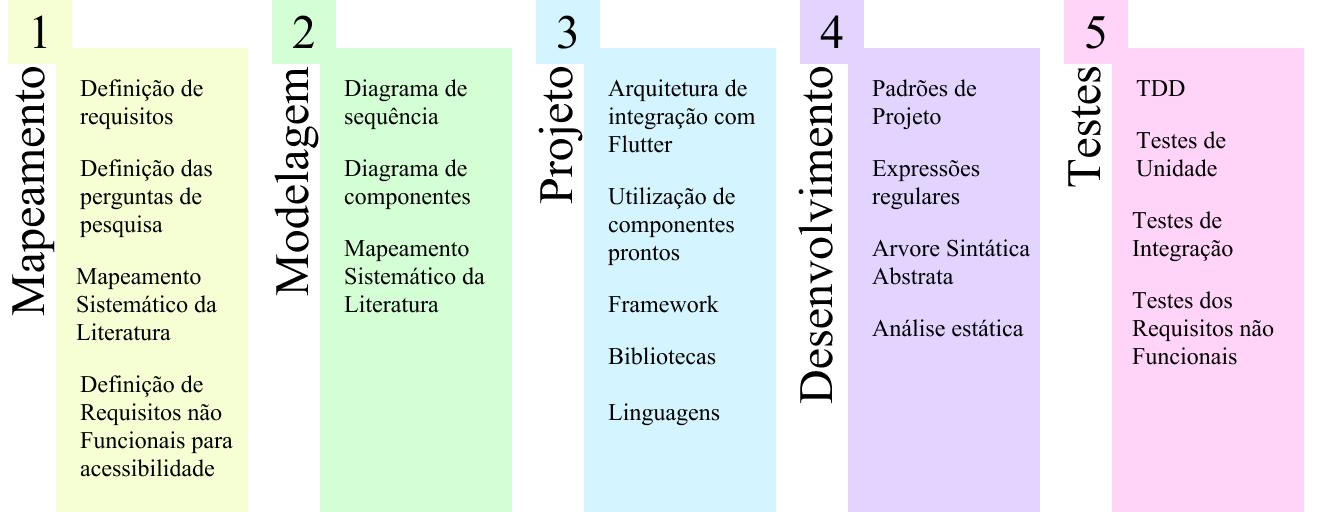
\includegraphics[scale=1]{Assets/Modelo de metodologia.png}
	\fonte{\me{2024}}
\end{figure}

A metodologia adotada permitiu um desenvolvimento estruturado e ágil do TCC, garantindo que a extensão proposta fosse construída de acordo com os requisitos de acessibilidade identificados. Além disso, a utilização do Scrum proporcionou flexibilidade e adaptabilidade durante o desenvolvimento, possibilitando ajustes e melhorias contínuas.

\section{Estrutura do trabalho}

O presente trabalho está organizado em capítulos que abordam os principais aspectos relacionados ao desenvolvimento da extensão proposta. A estrutura do trabalho é a seguinte:

\begin{itemize}
	\item Capítulo 2 - Revisão da Literatura: apresenta uma revisão da literatura sobre acessibilidade em aplicações móveis, abordando os principais conceitos, técnicas e ferramentas relacionadas ao tema.
	\item Capítulo 3 - Projeto e Implementação da Extensão: descreve o projeto e a implementação da extensão proposta, detalhando a arquitetura, as funcionalidades e as tecnologias utilizadas.
	\item Capítulo 4 - Testes e Validação: apresenta os testes e validações realizados com desenvolvedores e PCDs para avaliar a eficácia e a usabilidade da extensão.
	\item Capítulo 5 - Gerenciamento do Projeto: discute o gerenciamento do projeto, incluindo a metodologia ágil Scrum, as ferramentas utilizadas e os resultados obtidos.
	\item Capítulo 6 - Conclusões: apresenta as conclusões do trabalho, discutindo os principais resultados, limitações e possíveis trabalhos futuros relacionados ao tema da acessibilidade em aplicações móveis.
\end{itemize}